\chapter{\label{chap:cpsystems}\glsfmtname{cps}: \glsfmtname{ps} with Complex Symbols}

\gls{cps} is another variant of \gls{ps}, developed by Radu Nicolescu and collaborators in the early 2010s and complementary to the classic trinity of \gls{clps} \cite{Paun2000}, \gls{tlps} \cite{Martin-Vide2003}, and \gls{snps} \cite{Ionescu2006}.  It is largely based on \gls{clps} in that the core unit of it is the \emph{\gls{tlc}}, which is arranged as a nested tree structure and arguably can be seen, to some extent at least, as a higher-level abstraction over \gls{clps} \cite{Nicolescu2018}.  It can also incorporate elements of \gls{tlps}, in that \gls{cps} includes concepts of channels and message passing between \glspl{tlc} \cite{Henderson2019}, with an arbitrary number of these cells in the environment.  

A key difference from \gls{clps} and \gls{tlps}, however, is that in \gls{cps} \emph{only} the \glspl{tlc} have accompanying rules.  All subcells are merely inert symbolic objects operated upon by the \gls{tlc}'s rules.  These subcells are represented as labelled multisets within the \glspl{tlc}.  \citeauthor{Nicolescu2014a} demonstrated that not only is \gls{cps} capable of performing the same tasks as other \gls{ps} variants, but it also can be used to model standard computer programs \cite{Nicolescu2014a}.

This \namecref{chap:cpsystems} provides an overview of \gls{cps}.  Further presentation of \gls{cps} has appeared most recently in \cite{Nicolescu2018,Henderson2019,Henderson2020,Liu2020,Liu2021}, and it is recommended that the interested reader peruse those too.  While \gls{cps} is transitively bio-inspired through its basis in \gls{ps}, it has not been developed to simulate or model real-world biology.  Instead, it is intended as a useful theoretical model for computation.

% --------------------------------------------------
\section{A Partial History of \glsfmtname{cps}}

Since its inception, \gls{cps} has been studied and applied to various problems in computer science.  Indeed, it originated from the desire to find more expressive ways to present solutions to problems using \gls{mc}.  The root of \gls{cps}' evolution perhaps took seed in \cite{Balanescu2011}, which defined and used higher-level rules that can be seen as the progenitor of the style of rules characteristic of \gls{cps} today (see \vref{sec:cps:genericrules}).  This was followed by \cite{Nicolescu2012}, where variations upon more traditional \gls{ps} were further developed when considering parallel and distributed algorithms in \gls{mc}.

A systematic formalisation of this emerging new \gls{ps} variant was given in \cite{Nicolescu2014a}, which outlined the original basis of some aspects of \gls{cps} described in this \namecref{chap:cpsystems}.  Published contemporaneously with \cite{Nicolescu2014a} was \cite{Nicolescu2014}, which used \gls{cps} to demonstrate an effective implementation of \citeauthor{Guo1989}'s algorithm for ``image skeletonisation'' \cite{Guo1989}.

Subsequently, \gls{cps} was applied to a variety of problems, including a structured grid algorithm for region growing in greyscale images \cite{Nicolescu2015}; Byzantine Agreement \cite{Nicolescu2017}; and finding the most common words in a text corpus \cite{Nicolescu2018a}.  Throughout these, \gls{cps} was further refined and propounded.  These new developments were combined and summarised in \cite{Nicolescu2018}, which provided a central reference for the now-crystallised \gls{cps} variant.

Further developments have followed recently, describing \glspl{actor} in \gls{cps} \cite{Henderson2019};  solving a PSPACE-complete problem in linear time using \gls{cps} \cite{Henderson2020}; formal verification of \gls{cps} \cite{Liu2020,Liu2021a}; comparing Water Computing with \gls{cps} \cite{Henderson2021}; and an efficient algorithm for carrying out unification \cite{Liu2021} (see \cref{sec:cps:unification}), a missing piece of the puzzle regarding practical implementations.

\subsection{Specific Earlier Publications of this Chapter's Material}
This \namecref{chap:cpsystems} is believed to be the most comprehensive description of \gls{cps} to date, combining previous disparate work with original material.  As briefly outlined above, material on \gls{cps} has already been published in several articles.  Parts of this \namecref{chap:cpsystems} are new to this work, but other parts have been adapted from those earlier papers.  In particular:
\begin{itemize}
    \item \Cref{sec:cps:complexsymbols,sec:cps:highlevelrules,sec:cps:outsymbols,sec:cps:datastructures} were reproduced from \cite{Cooper2019}.
    \item A version of \cref{sec:cps:formaldescriptions} first appeared in \cite{Cooper2019a}.
    \item \Cref{sec:median:sortsets} was presented at the International Conference on Membrane Computing 2021 \cite{Cooper2021a}.
    \item \Cref{sec:cps:intertlcmess}, excluding \cref{sec:cps:outsymbols}, was written for \cite{Cooper2022}.  As were \cref{sec:cps:microsurg,sec:cps:compoundterms}.
\end{itemize}

Everything else contained in this \namecref{chap:cpsystems} but not mentioned above is original to this dissertation.

% --------------------------------------------------

\section{Advantages of \glsfmtname{cps}}
A significant advantage of \gls{cps} over traditional \gls{clps} is a simplification in the specification of complete systems to solve a given problem.  \Gls{clps} (as well as \gls{tlps} and \gls{snps}) typically require the definition of a uniform or semi-uniform family of \glspl{ruleset} customised to the specific instance of the problem at hand, whereas \gls{cps} normally requires only the definition of a fixed (usually much shorter) set of rules that cover all possible instances. As a result, only inputs to the system need to vary to solve different instances of the problem, \eg{} in \cref{chap:tsp} just five fixed rules are necessary to solve any instance of the \gls{tsp}, requiring only customisation of the input objects (in that case, elements describing the vertices and arcs of the digraph).

Equivalently, Dijkstra \cite{DijkstraWikiquote} said \blockquote{The purpose of abstracting is not to be vague, but to create a new semantic level in which one can be absolutely precise,} and, moreover, \blockquote{Our intellectual powers are rather geared to master static relations and \textelp{} our powers to visualize processes evolving in time are relatively poorly developed. For that reason we should do (as wise programmers aware of our limitations) our utmost to shorten the conceptual gap between the static program and the dynamic process, to make the correspondence between the program (spread out in text space) and the process (spread out in time) as trivial as possible.}.  These two quotes, while said in other contexts, also neatly sum up some key benefits of \gls{cps}.  The higher-level of \gls{cps} ensures that the systems' creator can concentrate only on details relevant to the matter, and elide organisational aspects that are largely mechanical, which can help said creator \enquote{see the forest for the trees.}  Furthermore, an intelligently constructed \glspl{cps} handles evolution through time near-automatically.  By and large, the designer need only specify the general process to follow in a certain state and the conditions marking a change in process, and delegate further responsibility for carrying those processes out to the \gls{cps} ``runtime'' itself.

The other key advantages of \gls{cps} are:
\begin{inparaenum}[a)]
\item that it often permits fairly direct, intelligible and brief translations into modern programming languages --- this is experimented with in various ways and with various languages throughout this dissertation; and,
\item that there appears to be great potential for highly efficient implementations of \gls{cps} algorithms for non-traditional hardware, though this is unexplored further here.
\end{inparaenum}

One might reasonably question \emph{how} \gls{cps} provides these claimed benefits.  The key is the use of \emph{variables} \& \emph{unification} and \emph{pattern matching}, all of which are inspired by logic programming and detailed below.  Variables and their unification enable the higher-level specifications of \gls{cps} by deferring the choice of the objects on which a given rule execution shall operate until the moment of execution.  Instead of requiring the designer to specify distinct rules to cover multitudinous possibilities, often a single rule can be made to adapt itself naturally to whatever may exist in the system at a given moment, by substituting those objects in for the variables as required.  Pattern matching is intrinsically linked to the other two, and further raises the level of abstraction.  It enables rules which focus specifically only on the relevant elements of objects present in a system, and ignore anything irrelevant to that context.

%-----------------------------------------------------------------------------------
\section{\label{sec:cps:complexsymbols}Complex Symbols as Subcells}
%-----------------------------------------------------------------------------------

\emph{Complex symbols} or \emph{subcells}, 
play the roles of cellular microcompartments or substructures,
such as organelles, vesicles, or cytoophidium assemblies (``snakes''),
which are embedded in cells or travel between cells, 
but without having the full processing power of a complete cell.
In \gls{cps}, subcells represent nested, labelled, data-only \glspl{compartment}
with no processing power of their own;
instead, the rules of their enclosing cells act upon them.
% instead, they are acted upon by the rules of their enclosing cells.

% Subcells can be either \emph{atoms} or \emph{compound terms}: multisets labelled by \emph{\glspl{functor}} (`\gls{functor}' is also commonly used as a shorthand for said compound terms).  Atoms, as the name suggests, are indivisible symbols.  They can be of any given type relevant to a system, but are static objects with no other inherent distinctive properties.  Atoms are written simply as the name of the atom's type.  Compound terms are objects that may contain both atoms and other compound terms and are written with the \gls{functor}'s type, followed by opening and closing parentheses, surrounding the encapsulated multiset.\footnote{For legibility, many compound terms in this work have been written with growing parentheses, dependent upon the level of nesting of terms involved.  This typesetting behaviour is not required or even specified as a part of \gls{cps} and can be freely omitted.}

%-------------------------------------------------------
\subsection{\label{sec:cps:terms}Subcells' Symbols} 
%-------------------------------------------------------

Subcells can be either \emph{atoms} or \emph{compound terms}: multisets labelled by \emph{\glspl{functor}} (`\gls{functor}' is also commonly used as a shorthand for said compound terms).  Atoms, as the name suggests, are indivisible symbols.  They can be of any given type relevant to a system, but are static objects with no other inherent distinctive properties.  Atoms are written simply as the name of the atom's type.  Compound terms are objects that may contain both atoms and other compound terms and are written with the \gls{functor}'s type, followed by opening and closing parentheses, surrounding the encapsulated multiset.\footnote{For legibility, many compound terms in this work have been written with growing parentheses, dependent upon the level of nesting of terms involved.  This typesetting behaviour is not required or even specified as a part of \gls{cps} and can be freely omitted.}

The basic vocabulary consists of atoms and \emph{variables}, collectively known as \emph{simple symbols}.  \emph{Complex symbols} are similar to Prolog-like \emph{first-order terms}, recursively built from \emph{multisets} of atoms and variables.  Together, complex symbols and simple symbols (atoms, variables) are called \emph{symbols} and can be defined by the following formal grammar:

\begin{framed}
\vspace{-0.6cm}
\begin{small}
\begin{bnf*}
    \bnfprod*{symbol}{\bnfpn{atom} \bnfor \bnfpn{variable} \bnfor \bnfpn{term}}\\
    \bnfprod*{term}{\bnfpn{functor} \bnfsp \bnfts{`('} \bnfsp \bnfpn{argument} \bnfsp \bnfts{`)'}}\\
    \bnfprod*{functor}{\bnfpn{atom}}\\
    \bnfprod*{argument}{\bnfes \bnfor \bnfsp \bnfpn{symbol} \bnfsp \bnfts{+}}
\end{bnf*}
\end{small}
\vspace{-0.8cm}
\end{framed}

Atoms are typically denoted by lower case letters (or, occasionally, digits), usually drawn from the Latin alphabet, 
such as \(a\), \(b\), \(c\), \(\cpundig\). 
Variables are typically denoted by upper case letters, 
such as \(X\), \(Y\), \(Z\).
\Eg{} an x atom may be written as \(x\), while a compound term labelled by a y \gls{functor} might be written as \(\cpfunc{y}{a \, xx \, z}\).  When there is more than one of a given atom present, the count is usually written as a superscript, so the earlier compound term would look like \(\cpfunc{y}{a \, x^2 \, z}\).  
\Glspl{functor} can only be atoms, not variables.

While not strictly necessary, one may also use \emph{anonymous variables} for improved readability, denoted by underscores (``\(\cpdiscard\)'').
Each underscore occurrence represents a \emph{new} unnamed variable
and indicates that something must fill that slot, but the specifics of what are unimportant.

Symbols that do \emph{not} contain variables are called \emph{ground}, \eg{}:
\begin{itemize}
\item Ground symbols:
\(a\), \(\cpfunc{a}{\cpempty}\), \(\cpfunc{a}{b}\), \(\cpfunc{a}{b c}\), \(\cpfunc{a}{b^2 c}\), \(\cpfunc{a}{\cpfunc{b}{c}}\), \(\cpfunc{a}{b\cpfunc{c}{\cpempty}}\), \(\cpfunc{a}{\cpfunc{b}{c}\cpfunc{d}{e}}\), \(\cpfunc{a}{\cpfunc{b}{c}\cpfunc{d}{e}}\), \(\cpfunc{a}{\cpfunc{b}{c}\cpfunc{d}{\cpfunc{e}{\cpempty}}}\), \(\cpfunc{a}{bc^2 d}\).

\smallskip
\item Symbols which are not ground:
\(X\), \(\cpfunc{a}{X}\), \(\cpfunc{a}{bX}\), \(\cpfunc{a}{\cpfunc{b}{X}}\), \(\cpfunc{a}{XY}\), \(\cpfunc{a}{X^2}\), \(\cpfunc{a}{XdY}\),  \(\cpfunc{a}{X\cpfunc{c}{}}\), \(\cpfunc{a}{\cpfunc{b}{X}\cpfunc{d}{e}}\), \(\cpfunc{a}{\cpfunc{b}{c}\cpfunc{d}{Y}}\), \(\cpfunc{a}{\cpfunc{b}{X^2}\cpfunc{d}{\cpfunc{e}{Xf^2}}}\);
also, using anonymous variables: \(\_\), \(\cpfunc{a}{b\_}\), \(\cpfunc{a}{X\_}\), \(\cpfunc{a}{\cpfunc{b}{X}\cpfunc{d}{\cpfunc{e}{\_}}}\).

\smallskip
\item This term-like construct which starts with a variable is \emph{not} a symbol (the above grammar defines first-order terms only):
\(\cpfunc{X}{a Y}\).
\end{itemize}

In \emph{concrete} models, cells contain ground symbols only.
Rules may, however, contain \emph{any} kind of symbols, atoms, variables, and terms (whether ground or not).

%-------------------------------------------------------
\subsection{\label{sec:cps:specialpurposeatoms}Special-purpose Atoms} 
%-------------------------------------------------------

There are two special atoms defined with specific meanings across \gls{cps}.  Empty multisets are denoted with \(\cpempty\), and instances of natural numbers with the \emph{counting atom} (see further \vref{sec:cps:natnums}).
One may abbreviate the expression of complex symbols by removing inner \(\cpempty\)'s as explicit references to the empty multiset, \eg{}~\(\cpfunc{a}{\cpempty} = \cpfunc{a}{\,}\).  Alternatively, where the term stores a number, \(\cpempty\) may instead be replaced with \(0\) (\ie{} the numeral for zero).

%-------------------------------------------------------
\subsection{\label{sec:cps:unification}Unification} 
%-------------------------------------------------------
All symbols which appear in rules (ground or not) can be (asymmetrically) \emph{matched} against \emph{ground} terms,
using an ad-hoc version of \emph{pattern matching}, 
more precisely, a \emph{one-way first-order syntactic unification} (one-way, because \glspl{tlc} may not contain variables) \cite{Liu2021}.
An atom can only match another copy of itself, but
a variable can match any multiset of ground terms (including \(\cpempty\)).
This may create combinatorial \emph{non-determinism}, 
when a combination of two or more variables are matched against the same multiset,
in which case an arbitrary matching is chosen. 
For example:
\begin{itemize}
\item Matching \(\cpfunc{a}{\cpfunc{b}{X}fY} = \cpfunc{a}{\cpfunc{b}{c\cpfunc{d}{e}}f^2g}\) deterministically creates a single set of unifiers:
\(X, Y = c\cpfunc{d}{e}, fg\).

\smallskip
\item Matching \(\cpfunc{a}{XY^2} = \cpfunc{a}{de^2f}\) deterministically creates a single set of unifiers: 
\(X, Y = df, e\).

\smallskip
\item Matching \(\cpfunc{a}{\cpfunc{b}{X}\cpfunc{c}{\cpundig X}} = \cpfunc{a}{\cpfunc{b}{\cpundig^2}\cpfunc{c}{\cpundig^3}}\) deterministically creates one single unifier: 
\(X = \cpundig^2\).

\smallskip
\item Matching \(\cpfunc{a}{\cpfunc{b}{X}\cpfunc{c}{\cpundig X}} = \cpfunc{a}{\cpfunc{b}{\cpundig^2}\cpfunc{c}{\cpundig^2}}\) fails.

\smallskip
\item Matching \(\cpfunc{a}{XY} = \cpfunc{a}{df}\) non-deterministically creates one of the following four sets of unifiers: 
\(X, Y = \cpempty, df\); \(X, Y = df, \cpempty\); \(X, Y = d, f\); \(X, Y = f, d\). 
\end{itemize}

% %-----------------------------------------
% \subsubsection{Performance Note}
% %-----------------------------------------
% If the rules avoid any matching non-determinism, 
% this proposal should not affect the performance of \gls{ps} simulators running on existing machines.
% Assuming that multisets/bags are already taken care of, \eg{}~via hash-tables,
% the proposed unification probably adds an almost linear factor.
% Recall that, in similar contexts (no occurs check needed), 
% Prolog unification algorithms can run in \(O(n g(n))\) steps,
% where \(g\) is the inverse Ackermann function.
% This conjecture must be proven, though, 
% as the novel presence of multisets may affect the performance.

% % -------------------------------------------------
%-----------------------------------------------------------------------------------
\section{\label{sec:cps:highlevelrules}High-level or Generic Rules}
%-----------------------------------------------------------------------------------

%-------------------------------------------------------
\subsection{\label{sec:cps:genericrules}Generic Rules Format}
%-------------------------------------------------------
% Consider rules of the following \emph{generic} format 
% (called generic because it defines templates involving variables):
% \begin{framed}
% \vspace{-0.6cm}
% \begin{align*}
% \textsf{current-state} ~~ \textsf{symbols} \dots ~ \rightarrow_\alpha ~ & \textsf{target-state} ~~ (\textsf{in-symbols}) \dots ~~ \\
%  & (\textsf{out-symbols})_\delta \dots \\
%  & | ~  \textsf{\glspl{promoter}} \dots ~~ \neg ~  \textsf{\glspl{inhibitor}} \dots
% \end{align*}
% \vspace{-0.8cm}
% \end{framed}
% Where:
% \begin{itemize}
% \item \textsf{current-state} and \textsf{target-state} are atoms or terms;  these are traditionally written in the form \(s_x\) where \(x\) is a sequential numeral (\eg{} \(s_1\), \(s_2\) \etc{}), but any valid ground atom or term as appropriate is permitted.

% \smallskip
% \item \textsf{symbols}, \textsf{in-symbols}, \textsf{\glspl{promoter}} and \textsf{\glspl{inhibitor}} are symbols;

% \smallskip
% \item \textsf{in-symbols} become available after the end of the current step only, as in traditional \gls{ps}  (one can imagine that these are sent via an \adhoc{} fast \textsf{loopback} channel); 

% \smallskip
% \item subscript \(\alpha\) \(\in\) \(\{\cponce\), \(\cpmaxpar\}\), 
% indicates the application mode, discussed further in \cref{sec:cps:applicationmodes};

% \smallskip
% \item \textsf{out-symbols} are sent to the cell's structural neighbours at the end of the step.
% These symbols are enclosed in angle brackets that indicate 
% their destinations, abbreviated above as \(\delta\). 
% The most usual scenarios include: 

% \begin{itemize}
% \item \(\cpoutsymbol{a}{i}\) indicates that \(a\) is sent over outgoing arc \(i\) (unicast); 

% \item \(\cpoutsymbol{a}{i,j}\) indicates that \(a\) is sent over outgoing arcs \(i\) and \(j\)(multicast); 

% \item \(\cpoutsymbolall{a}\) indicates that \(a\) is sent over all outgoing arcs (broadcast). 
% \end{itemize}

% All symbols sent via one \emph{generic rule} to the same destination form one single \emph{message}, and they travel together as one single block (even if the generic rule is applied in mode \(\cpmaxpar\)).
% \end{itemize}

Consider rules of the following \emph{generic} format 
(called generic because it defines templates involving variables):
\begin{framed}
\vspace{-0.6cm}
\begin{align*}
 current-state  ~~  symbols  \dots ~ \rightarrow_\alpha ~ &  target-state  ~~ ( in-symbols ) \dots ~~ \\
 & | ~  \glspl{promoter} \dots ~~ \neg ~  \glspl{inhibitor} \dots
\end{align*}
\vspace{-0.8cm}
\end{framed}
Where:
\begin{itemize}
\item  current-state  and  target-state  are atoms or terms;  these are traditionally written in the form \(s_x\) where \(x\) is a sequential numeral (\eg{} \(s_1\), \(s_2\) \etc{}), but any valid ground atom or term as appropriate is permitted.

\smallskip
\item  symbols, \glspl{promoter} and \glspl{inhibitor} are symbols;

\smallskip
\item  in-symbols  become available after the end of the current step only, as in traditional \gls{ps}  (one can imagine that these are sent via an \adhoc{} fast  loopback  channel); 

\smallskip
\item subscript \(\alpha\), \(\{\cponce\), \(\cpmaxpar\}\), 
indicates the application mode, discussed further in \cref{sec:cps:applicationmodes};

% \smallskip
% \item \textsf{out-symbols} are sent to the cell's structural neighbours at the end of the step.
% These symbols are enclosed in angle brackets that indicate 
% their destinations, abbreviated above as \(\delta\). 
% The most usual scenarios include: 

% \begin{itemize}
% \item \(\cpoutsymbol{a}{i}\) indicates that \(a\) is sent over outgoing arc \(i\) (unicast); 

% \item \(\cpoutsymbol{a}{i,j}\) indicates that \(a\) is sent over outgoing arcs \(i\) and \(j\)(multicast); 

% \item \(\cpoutsymbolall{a}\) indicates that \(a\) is sent over all outgoing arcs (broadcast). 
% \end{itemize}

% All symbols sent via one \emph{generic rule} to the same destination form one single \emph{message}, and they travel together as one single block (even if the generic rule is applied in mode \(\cpmaxpar\)).
\end{itemize}

%-------------------------------------------------------
\subsection{Pattern Matching}
%-------------------------------------------------------
Rules are matched against \gls{tlc} contents using the aforementioned \emph{pattern matching},
which involves the rule's \emph{\gls{lhs}}, \glspl{promoter} and \glspl{inhibitor}.

Generally, variables have \emph{global rule scope};
these are assumed to be introduced by \emph{existential} quantifiers preceding the rule
--- except for \glspl{inhibitor}, which may introduce \emph{local variables}, 
as further discussed in \vref{sec:cps:prominhi}. 

The matching is \emph{valid} only if, after unification/substituting variables by their values, 
the rule's \emph{\gls{rhs}} contains ground terms only
(so \emph{no} free variables are injected in the \gls{tlc} or sent to its neighbours),
as illustrated by the following sample scenario:
\begin{itemize}
\item The cell's \emph{current content} includes the \emph{ground term}:\\
\(\cpfunc{n}{a \, \cpfunc{\phi}{b \, \cpfunc{\phi}{c} \, \cpfunc{\psi}{d}} \, \cpfunc{\psi}{e}}\)

\smallskip
\item The following (state-less) \emph{rewriting rule} is considered: \\ 
\(\cpfunc{n}{X \, \cpfunc{\phi}{Y \, \cpfunc{\phi}{Y_1} \, \cpfunc{\psi}{Y_2}} \, \cpfunc{\psi}{Z}} ~ \rightarrow ~ \cpfunc{v}{X} \: \cpfunc{n}{Y \, \cpfunc{\phi}{Y_2} \, \cpfunc{\psi}{Y_1}} \: \cpfunc{v}{Z}\)

\smallskip
\item The pattern matching determines the following \emph{unifiers}: \\
\(X = a\), \(Y = b\), \(Y_1 = c\), \( Y_2 = d\), \(Z = e\).

\smallskip
\item This is a \emph{valid} matching and, after \emph{substitutions}, 
the rule's \gls{rhs} gives the \emph{new content}: \\
\(\cpfunc{v}{a} ~ \cpfunc{n}{b \, \cpfunc{\phi}{d} \, \cpfunc{\psi}{c}} ~ \cpfunc{v}{e}\)
\end{itemize}

%-------------------------------------------------------
\subsection{\label{sec:cps:prominhi}Promoters and Inhibitors}
%-------------------------------------------------------

Promoters are objects that \emph{must} be present within the \gls{tlc} for the rule to be applicable but are \emph{not} removed by the rule.  Conversely, \glspl{inhibitor} are objects that \emph{must not} be present for the rule to be applicable, although the rule may create them.  If \glspl{promoter} are present, they are denoted following a \(|\) per \gls{promoter}, and \glspl{inhibitor} by \(\neg\), \eg{} \(|\,\cpfunc{a}{A}\) or \(\neg\,\cpfunc{b}{B}\).  Promoters and \glspl{inhibitor} are traditionally written below the main rule body, but this is not strictly required.  Promoters are typically written first, followed by \glspl{inhibitor}, but this too is not compulsory.  All \glspl{promoter} and \glspl{inhibitor} have equal priority among themselves for a given attempted unification of a rule.

\lstset{xleftmargin=.5in, xrightmargin=.5in} 
\begin{lstlisting}
  $| ~ \cpfunc{a}{A}$ #\hfill \gls{promoter} \enspace#
  $\neg ~ \cpfunc{b}{B}$ #\hfill \gls{inhibitor} \enspace#
\end{lstlisting}

To define additional useful matchings expressively, 
\glspl{promoter} and \glspl{inhibitor} may also use virtual ``equality'' terms, 
written in infix format, with the \(=\) operator.
For example, including the term \((ab = XY)\) indicates the following additional matching constraints on variables \(X\) and \(Y\): either \(X, Y = ab, \cpempty\); or \(X, Y = a, b\); or \(X, Y = b, a\); or \(X, Y = \cpempty, ab\).

To define \glspl{inhibitor} as logical negations usefully,
variables that only appear in the scope of an \gls{inhibitor} are assumed to have \emph{local scope}. 
Furthermore, these variables are assumed to be defined by \emph{existential} quantifiers, immediately after the negation. 
Semantically, this is equivalent to introducing these variables at the global rule level, 
but by \emph{universal} quantifiers, after all other global variables;
introduced by \emph{existential} quantifiers.

As an illustration, consider a \gls{tlc} containing \(\cpfunc{a}{c} ~ \cpfunc{a}{ccc}\) and contrast two rules, 
containing the following two sample \gls{promoter}/\gls{inhibitor} pairs 
(for brevity, other rule details are omitted here).

\lstset{xleftmargin=.5in, xrightmargin=.5in} 
\begin{lstlisting}
... $\mid$  $\cpfunc{a}{cXY}$     $\neg$  $\cpfunc{a}{X}$    #\hfill (1)\enspace#
... $\mid$  $\cpfunc{a}{cZ}$     $\neg$  $(Z=XY)$  $\cpfunc{a}{X}$    #\hfill (2)\enspace#
\end{lstlisting}

These two rules appear very similar, and their \gls{inhibitor} tests share the same expression: 
\emph{No} \(\cpfunc{a}{X}\) may be present in the \gls{tlc}.

Rule (1) uses two global variables, \(X, Y\). 
According to its \gls{promoter}, \(\cpfunc{a}{cXY}\), these variables can be matched in four different ways:
(1a) \(X, Y = \cpempty, \cpempty\); (1b) \(X, Y = cc, \cpempty\); (1c) \(X, Y = \cpempty, cc\); (1d) \(X, Y = c, c\).\footnote{Strictly speaking, this matching is possible in multiple ways, with different \(c\) atoms assigned to each variable.  For current purposes, though, they are equivalent and so are reduced to the one result.}
Three different unifications, (1a), (1b), (1c), pass the \gls{inhibitor} test, 
as there are no cell terms \(\cpfunc{a}{\,}\), \(\cpfunc{a}{cc}\), \(\cpfunc{a}{\,}\), respectively. 
Unification (1d) fails the \gls{inhibitor} test because there \emph{is} one cell term \(\cpfunc{a}{c}\).

Rule (2) uses one global variable, \(Z\), and two local \gls{inhibitor} variables, \(X, Y\).
According to its \gls{promoter}, \(\cpfunc{a}{cZ}\), variable \(Z\) can be matched in two different ways: 
(2a) \(Z = \cpempty\); (2b) \(Z = cc\).
Unification (2a) passes the \gls{inhibitor} test because it only generates one local unification,
\(X, Y = \cpempty, \cpempty\), and there is \emph{no} cell term \(\cpfunc{a}{\,}\).
Unification (2b) fails the \gls{inhibitor} test because it generates all three following local unifications:
(2b1) \(X, Y = cc, \cpempty\); (2b2) \(X, Y = \cpempty, cc\); (2b3) \(X, Y = c, c\); 
and there \emph{is} a cell term corresponding to (2b3), \(\cpfunc{a}{c}\).

%-------------------------------------------------------
\subsection{\label{sec:cps:applicationmodes}Application Modes: Exactly-once and Maximally-parallel}
%-------------------------------------------------------
To explain the two rule application modes, \(\cponce\) and \(\cpmaxpar\) (referred to as \emph{exactly-once} and \emph{maximally-parallel} respectively) consider a \gls{tlc}, \(\sigma\), containing three counter-like complex symbols,
\(\cpfunc{c}{\cpundig^2}\), \(\cpfunc{c}{\cpundig^2}\), \(\cpfunc{c}{\cpundig^3}\),
and the two possible application modes of the following high-level ``decrementing'' rule:
\vspace{-0.2cm}
\begin{framed}
\vspace{-0.5cm}
\[(\rho_\beta) ~s_1 ~\cpfunc{c}{\cpundig \, X} \rightarrow_{\alpha} s_2 ~\cpfunc{c}{X},\\
\mathrm{where} \; \alpha \in \{\cponce, \cpmaxpar\}.\]
\vspace{-0.8cm}
\end{framed}

% The \gls{lhs} of rule \(\rho_\beta\), \(\cpfunc{c}{\cpundig \, X}\), can be unified in three different ways,
% to each one of the three \(c\) symbols extant in cell \(\sigma\).
% Conceptually, this rule may be instantiated in three different ways,
% each one tied and applicable to a distinct symbol:
Conceptually, the \gls{lhs} of rule \(\rho_\beta\), \(\cpfunc{c}{\cpundig \, X}\), can be unified in three different ways,
to each one of the three distinct \(c\) compound symbols extant in \gls{tlc} \(\sigma\):
% Conceptually, this rule may be instantiated in three different ways,
% each one tied and applicable to a distinct symbol:
\begin{eqnarray*}
& (\rho_1)  & ~s_1 ~\cpfunc{c}{\cpundig^2} \rightarrow_{\alpha} s_2 ~\cpfunc{c}{\cpundig},\\
& (\rho_2)  & ~s_1 ~\cpfunc{c}{\cpundig^2} \rightarrow_{\alpha} s_2 ~\cpfunc{c}{\cpundig},\\
& (\rho_3) & ~s_1 ~\cpfunc{c}{\cpundig^3} \rightarrow_{\alpha} s_2 ~\cpfunc{c}{\cpundig^2}.
\end{eqnarray*}

\begin{enumerate}
\item If \(\alpha = \: \cponce\), rule~\(\rho_1\) 
non-deterministically selects and applies one of these virtual rules \(\rho_1\), \(\rho_2\), \(\rho_3\).
Using \(\rho_1\) or \(\rho_2\), 
cell \(\sigma\) ends with counters \(\cpfunc{c}{\cpundig}\), \(\cpfunc{c}{\cpundig^2}\), \(\cpfunc{c}{\cpundig^3}\).
Using \(\rho_3\),
cell \(\sigma\) ends with counters \(\cpfunc{c}{\cpundig^2}\), \(\cpfunc{c}{\cpundig^2}\), \(\cpfunc{c}{\cpundig^2}\).

\smallskip
\item If \(\alpha = \: \cpmaxpar\), rule~\(\rho_\cpmaxpar\) 
applies in parallel all these virtual rules \(\rho_1\), \(\rho_2\), \(\rho_3\).
Cell \(\sigma\) ends with counters \(\cpfunc{c}{\cpundig}\), \(\cpfunc{c}{\cpundig}\), \(\cpfunc{c}{\cpundig^2}\).
\end{enumerate}

Semantically, the \(\cpmaxpar\) mode is equivalent to a virtual sequential \texttt{while} loop around the same rule in \(\cponce\) mode, which is repeated until it is no longer applicable.  All such applications of the rule are carried out concurrently in a single step, however.

Like most other \gls{ps} variants, \gls{cps} ordinarily evolve synchronously in a stepwise fashion following an implicit global clock.  Rules are applied based on whether the available multiset(s) within the system match the rules' \gls{lhs} and \glspl{promoter}, and not the \glspl{inhibitor}.  The consumption of removed objects plus the creation of new objects happens instantaneously at the end of a step.

%-------------------------------------------------------
\subsection{Benefits}
%-------------------------------------------------------
This type of generic rules allows
\begin{inparaenum}[(i)]
\item a reasonably fast parsing and processing of subcomponents; and
\item algorithm descriptions with \emph{fixed-size alphabets} and \emph{fixed-sized \glspl{ruleset}}, 
independent of the size of the problem and the number of \glspl{tlc} in the system (often \emph{impossible} with only atomic symbols).
\end{inparaenum}

%-------------------------------------------------------
\subsection{Special Cases}
%-------------------------------------------------------
Simple scenarios involving generic rules are sometimes 
semantically equivalent to sets of non-generic (ground) rules defined via bounded loops.
For example, consider the rule
\[
s_1 ~ \cpfunc{a}{IJ} ~ \rightarrow_\cpmaxpar ~ s_2 ~ \cpfunc{b}{I} ~ \cpfunc{c}{J},
\]
where the \gls{tlc}'s contents guarantee that \(I\) and \(J\) 
only match integers in ranges \([1,n]\) and \([1,m]\), respectively.
Under these assumptions, 
this rule is equivalent to the following set of non-generic rules:
\[
s_1 ~ a_{i,j} ~ \rightarrow s_2 ~ b_i ~ c_j, ~ \forall i \in [1,n], j \in [1,m].
\]

However, unification is a much more powerful concept, 
which cannot be reduced generally to simple bounded loops.
%-----------------------------------------------------------------------------------
\section{Inter-\glsentrytext{tlc} messaging}
%-----------------------------------------------------------------------------------

\Glspl{tlc} may exchange messages over channels (differently to the behaviour of out-symbols described in \cref{sec:cps:genericrules}).  Each \gls{tlc} may hold one or more appropriately labelled endpoints for any relevant channels, and may attempt both to send and to receive messages via those endpoints in its rules.  A message is written encapsulated inside angle brackets and marked with either an exclamation mark on the \gls{rhs} or a question mark on the \gls{lhs} to represent sending or receiving, respectively.  \Eg{} \(\cpsend{\cpfunc{a}{b}}{c}\) would represent a message \(\cpfunc{a}{b}\) to be sent via channel \(c\), and \(\cprecv{\cpfunc{d}{e}}{f}\) would represent a message to be received via channel \(f\).

Both sending and receiving use pattern matching.  For the sending case, any \gls{cps} term which matches the pattern in the rule may be removed from the \gls{tlc} and placed into a buffer multiset at the other end of the channel.  Receiving works similarly in that any object stored in the channel's nearby buffer multiset, which matches the pattern of a receipt rule, may be withdrawn.  If more than one object in the buffer matches the pattern, one of them is selected non-deterministically.  Importantly, this means that ordinary \gls{cps} channels do \emph{not} operate as FIFO queues by default.

\lstset{xleftmargin=.5in, xrightmargin=.5in} 
\begin{lstlisting}
  $\cpsend{\cpfunc{a}{b}}{c}$ #\hfill\textsl{send}\enspace#
  $\cprecv{\cpfunc{d}{e}}{f}$ #\hfill\textsl{receive}\enspace#
\end{lstlisting}

%-------------------------------------------------------
\subsection{\label{sec:cps:antiport}Antiport communication rules in \glsentrytext{cps}}
%-------------------------------------------------------

% We use an antiport rule \cite{Orellana-Martin2019,Paun2002} in \cref{sec:nmp:systemwide}.  In brief, antiport rules allow for the bidirectional exchange of objects between membranes/cells/neurons during a single rule execution, with the restriction that objects \emph{must} travel in both directions.  Thus, if one side is only ready to send or receive, rather than both, the rule cannot run at the next step.  An important ramification of this is that it prevents deadlock from both sides of the exchange waiting on the other to send a message.

Antiport rules \cite{Orellana-Martin2019,Paun2002} allow for the bidirectional exchange of objects between membranes/cells/neurons during a single rule execution, with the restriction that objects \emph{must} travel in both directions.  Thus, if one side is only ready to send or receive, rather than both, the rule cannot run at the next step.  An important ramification of this is that it prevents deadlock from both sides of the exchange waiting on the other to send a message.

% In the context of \gls{cps}, this means that a given rule must involve receipt over a channel on the left-hand-side, and sending on the \emph{same} channel on the right-hand-side.  For example, in the context of inter-\gls{tlc} messaging, \cpruleinline{ \cprule*{s_1}{\cpantirecv{\cpfunc{a}{B}}{c} \; \cpfunc{d}{E}}{1}{s_2}{\cpantisend{\cpfunc{d}{E}}{c} \; \cpfunc{a}{B}}} would be valid because the same channel is used on both sides of the rule.  To emphasise that the rule requires antiport behaviour, the sending and receiving terms have an extra ? or !, respectively.

In the context of \gls{cps}, this means that a given rule must involve receipt over a channel on the left-hand-side, and sending on the \emph{same} channel on the right-hand-side.  To emphasise that the rule requires antiport behaviour, the sending and receiving terms have an extra ? or !, respectively.

\lstset{xleftmargin=.5in, xrightmargin=.5in} 
\begin{lstlisting}
  $\cpantisend{\cpfunc{a}{b}}{c}$ #\hfill\textsl{antiport send}\enspace#
  $\cpantirecv{\cpfunc{d}{e}}{f}$ #\hfill\textsl{antiport receive}\enspace#
\end{lstlisting}

For example, \cpruleinline{ \cprule*{s_1}{\cpantirecv{\cpfunc{a}{B}}{c} \; \cpfunc{d}{E}}{1}{s_2}{\cpantisend{\cpfunc{d}{E}}{c} \; \cpfunc{a}{B}}} would be valid because the same channel is used on both sides of the rule.

\begin{anfxwarning}
A ramification of antiport communication is arguably that it completely bypasses the multisets at either end of the channel.  Whether this makes any practical difference is another story altogether.
\end{anfxwarning}

%-------------------------------------------------------
\subsection{\label{sec:cps:blocking}Blocking vs. non-blocking message receipt in \glsentrytext{cps}}
%-------------------------------------------------------

In \gls{cps} all outgoing communications from a \gls{tlc} to others is non-blocking by default.  The channels connecting the cells buffer message objects if needed, and thus an outgoing message can always be accepted by the channel even if the holder of the other end of the channel is not yet ready to receive the message.  Receiving messages via channels is also ordinarily a non-blocking operation in \gls{cps}, albeit for a different reason.  If there are no eligible messages on the channel, either buffered by the channel itself or offered by the cell holding the other end of the channel, then the rules to receive over that channel will not apply at the next step regardless of whichever other rules may or may not be applied.

It may be helpful in some circumstances, however, to simulate the nature of a blocking receipt.  This can be achieved with the use of additional dedicated states.  The beginning state for the intended blocking receipt should be unused as the beginning state for any other rule (except for another aspect of the same blocking receipt).  This state is also used as the ending state for another rule, which either is the end of another process in the computation or used as a test to determine whether to enter into a blocking receipt.  The ending state for the blocking receipt rule should return the cell to its standard process.

The overall effect of using the unique state is that it ensures no other rule may be used inside a particular \gls{tlc} at a given step.  Effectively, the \gls{tlc} becomes quiescent until another \gls{tlc} makes an appropriate offer to send a message to the first cell.  At that point, one or more messages are exchanged as appropriate, and the receiving \gls{tlc} returns to its standard processing otherwise.  This is used in \cref{sec:nmp:pespecific} (rules 9 \& 10 in \cref{ruleset:nmp:proxspec}).

% -------------------------------------------------
%-----------------------------------------------------------------------------------
\section{\label{sec:cps:formaldescriptions}Formal \glsfmtname{cps} Descriptions}
%-----------------------------------------------------------------------------------

A specific \glspl{cps} can be described by a 6-tuple, as shown below.

\[
\Pi_{cP}(T, A, O, R, S, \bar{s})
\]

\(T\) is the set of \glspl{tlc} at the start of the evolution of the system; \(A\) is the alphabet of the system; \(O\) is the set of multisets of initial objects in the \glspl{tlc}; \(R\) is the set of \glspl{ruleset} for each \gls{tlc}; \(S\) is the set of possible states of the \glspl{tlc}; and \(\bar{s} \in S\) is the starting state of every \gls{tlc} in the system.\footnote{Historically, many (perhaps most) presented \gls{cps} have used only a single \gls{tlc}.  Thus, any distinction between the state of the \gls{tlc} and the state as a whole has been irrelevant, meaning often times the system overall has been described as having a state, but this is inaccurate.}

Typically in practice, in the case of multiple \glspl{tlc} the same single ruleset \(R\) is used for every \gls{tlc} in the defined system.  In these cases, a single ruleset may be specified, which is assumed to apply to every \gls{tlc}.  Furthermore, strictly speaking, the symbols used to represent the states of the system are a part of the alphabet of the system.  Ordinarily they are not used for any other purpose, however, and so their specification is omitted from that of the alphabet \(A\).  \Ie{} if \(A_\alpha\) is the complete alphabet, the alphabet typically presented in the tuple is \( A_\beta = A_\alpha \setminus S \).
\section{Micro-surgeries on \glsentrytext{cps} \glsentrytext{tlc}s}
\subsection{A Problem}
A \gls{cps} cell can contain an arbitrary number of various objects, like other \gls{ps} variants.  A key difference between \gls{cps} and other variants, however, is that \gls{cps} can use one fixed-size \gls{ruleset} that applies to every possible initial multiset, while other variants typically require the definition of a family of related \glspl{ruleset} that change depending on the initial multiset present in the system.

This capacity for fixed-size \glspl{ruleset} is enabled primarily through the use of variables and unification, permitting the rules to adapt to the contents of the cells.  This tends to be an all-or-nothing situation, though, in that a single variable usually matches to the entire contents of whichever cell or functor it is specified in.  In the case of two or more variables in the same space, the split of the objects between them is made non-deterministically (per \cref{sec:cps:unification}), and may even be done such that one of the variables is empty.  Anything to be excluded from matching with a variable \emph{must} be listed explicitly, while anything remaining to be excluded from the operation of the rule entirely is covered with the underscore \emph{discard} (aka `don't care') symbol (\(\cpdiscard\)).  This is fine for many cases, but falls short in instances when there will be an unknown quantity of a given object in a cell, and it is not desirable to perform a single operation across all of them as one.

% As an example, consider a situation where there are an unknown number of \(d\) objects in the \gls{tlc}, and it is desirable to perform an operation for each of them.  Let there be an \(a\) functor containing four \(b\) objects, and a \(c\) functor containing three \(d\) objects, i.e. we have \(a(b^4)\) and \(c(d^3)\).  The goal is to write a rule that shall replicate the contents of \(a\) and place them inside a new \(e\) functor, and do this once per \(d\) present inside \(c\).  Once completed, \(a\) and \(c\) will hold their original contents immediately before the execution of the rules.

% Intuitively, if this operation is carried out as described, then the ending state of the system should be that it contains \(a(b^4)\), \(c(d^3)\) and \(e(b^{12})\).  This \emph{could} be achieved using rules as shown in \cref{rules:cps:slowmulti}.  While this would work, it requires steps equal to the size of the contents of \(c\) (i.e. three steps), as well as necessitating an uninteresting auxiliary rule.  Minor variations are possible, primarily regarding the choice of use of promoters, inhibitors and states, but ultimately, they would lead to roughly the same set.

As an example, consider a situation where there are an unknown number of \(d\) objects in the \gls{tlc}, and it is desirable to perform an operation for each of them.  Let there be an \(a\) functor containing four \(b\) objects, and a \(c\) functor containing three \(d\) objects, i.e. \(\cpfunc{a}{b^4}\) and \(\cpfunc{c}{d^3}\).  The goal is to write a rule that shall replicate the contents of \(a\) and place them inside a new \(e\) functor, and do this once per \(d\) present inside \(c\).  Once completed, \(a\) and \(c\) will hold their original contents from before the execution of the rules.

Intuitively, if this operation is carried out as described, then the ending state of the \gls{tlc} should be that it contains \(\cpfunc{a}{b^4}\), \(\cpfunc{c}{d^3}\) and \(\cpfunc{e}{b^{12}}\).  This \emph{could} be achieved using rules as shown in \cref{rules:cps:slowmulti}.  While this would work, it requires steps equal to the size of the contents of \(c\) plus one (i.e. four steps), as well as necessitating an uninteresting auxiliary rule.  Minor variations are possible, primarily regarding the choice of use of promoters, inhibitors and states, but ultimately, they would lead to roughly the same set.

\begin{cprulesetfloat}
    \begin{cpruleset}
        \cprule{s_0}{}{\cponce}{s_1}{\cpfunc{e}{\cpempty}~\cpfunc{f}{D}}
        \cppromoter{\cpfunc{c}{D}}
        
        % \cprule{s_1}{c(dD)~e(E))}{\cponce}{s_1}{c(D)~e(EB)}
        % \cppromoter{a(B)}
        
        \cprule{s_1}{\cpfunc{c}{dD} \; \cpfunc{e}{E}}{\cponce}{s_1}{\cpfunc{c}{D} \; \cpfunc{e}{EB}}
        \cppromoter{\cpfunc{a}{B}}
    
        % \cprule{s_1}{c(\cpempty)~f(D)}{\cponce}{s_2}{c(D)}
        \cprule{s_1}{\cpfunc{c}{\cpempty} \; \cpfunc{f}{D}}{\cponce}{s_2}{\cpfunc{c}{D}}
    \end{cpruleset}
    \caption[Simulation of multiplication in cP systems]{\label{rules:cps:slowmulti}Simulation of multiplication in cP systems.  The values in the \(a\) and \(c\) complex terms are multiplied, with the result stored in the \(e\) term}
\end{cprulesetfloat}

\begin{figure}
    \centering
    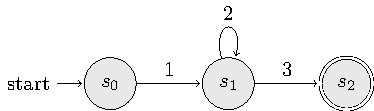
\includegraphics{chapters/cpsystems/ruleset1statemachine.pdf}
    \caption[State machine diagram for the system in \cref{rules:cps:slowmulti}]{State machine diagram for the system in \cref{rules:cps:slowmulti}.  Nodes are labelled with states, and edges with rules transitioning between them}
    \label{fig:cps:slowmulti}
\end{figure}

In particular, it is not possible here to make the second rule work in parallel --- a given functor or atom may only be used in one rule application per system step, and so the first rule application would take exclusive control of both the \(c\) functor and its \(d\) contents, preventing any further rule applications from occurring.  A further wrinkle of this \gls{ruleset} is the fact that it requires an extra temporary functor, \(f\), to store copies of the \(d\) atoms for transfer back into \(c\) at the end because the appropriate termination point for these rules can only be detected when \(c\) has been emptied.

\subsection{A Solution}
To avoid this problem, we revisit and clarify an older and rarely used operation that permits a rule to be applied to the contents of a sub-cell or functor, \emph{without} also seizing control (i.e. locking) of the sub-cell or functor itself.  We term this operation \emph{\gls{ms}}, representing the idea that as-minimal-as-possible modification is made to the containing object while modifying its contents.  We denote \glspl{ms} through the use of curly braces, rather than the usual parentheses for complex terms.  They are still complex terms, but the operation performed on them differs.  Due to this differing operation, every instance of a \gls{ms} on the \gls{lhs} \emph{must} have a matching instance on the \gls{rhs}.

% \cpruleinline{
% \cprule*{s_0}{}{\cponce}{s_1}{\cpfunc{e}{\cpempty}}
% \cprule*{s_1}{\cpfuncms{e}{\cpempty}}{\cpmaxpar}{s_2}{\cpfuncms{e}{B}~|~\cpfunc{c}{d\cpdiscard}~|~\cpfunc{a}{B}}}

% \begin{cprulesetfloat}
%     \begin{cpruleset}
%         \cprule{s_0}{}{\cponce}{s_1}{\cpfunc{e}{\cpempty}}

%         \cprule{s_1}{\cpfuncms{e}{\cpempty}}{\cpmaxpar}{s_2}{\cpfuncms{e}{B}}
%         \cppromoter{\cpfunc{c}{d\cpdiscard}}
%         \cppromoter{\cpfunc{a}{B}}
%     \end{cpruleset}
%     \caption{\label{rules:cps:microsurg}Rules for a destructive multiplication process that requires exactly two steps regardless of the numbers multiplied by using \gls{cps} \glspl{ms}}
% \end{cprulesetfloat}

\begin{cprulesetfloat}
    \begin{cpruleset}
        \cprule{s_0}{}{\cponce}{s_1}{\cpfunc{e}{\cpempty}}

        \cprule{s_1}{\cpfuncms{e}{\,}}{\cpmaxpar}{s_2}{\cpfuncms{e}{B}}
        \cppromoter{\cpfunc{c}{d\cpdiscard}}
        \cppromoter{\cpfunc{a}{B}}
    \end{cpruleset}
    \caption{\label{rules:cps:microsurg}Rules for a destructive multiplication process that requires exactly two steps regardless of the numbers multiplied by using \gls{cps} \glspl{ms}}
\end{cprulesetfloat}

\Cref{rules:cps:microsurg} is an example of three rules using \glspl{ms} that achieve in \emph{two} steps the same destructive multiplication as the \gls{ruleset} listed in \cref{rules:cps:slowmulti}, which requires \(D + 1\) steps.  Crucially, the second rule is still \emph{one} rule application, but the insertion of \(B\) into \(e\) happens once for each possible match on the promoter.  The use of \(c(d\cpdiscard)\) combined with the maximally parallel rule mode means that the rule will take control of and execute once for each \(d\) atom in the multiset labelled by the \(c\) functor.  As such, three lots of \(B\) will be inserted into \(e\) simultaneously while executing this rule under the example described above.

% Furthermore, non-destructive division of \(d\) by \(e\), \(d \div e = f\), could be:
% \cpruleinline{\cprule*{s_1}{\cpfuncms{f}{\cpempty}~\cpfuncms{d}{E}}{\cpmaxpar}{s_1}{f[\cpundig]~\cpfuncms{d}{\cpempty}~|~\cpfunc{e}{E}}}

% Furthermore, destructive division of \(d\) by \(e\), \(d \div e = f\), could be:
% \cpruleinline{\cprule*{s_1}{\cpfuncms{f}{\cpempty}~\cpfuncms{d}{E}}{\cpmaxpar}{s_1}{\cpfuncms{f}{\cpundig}~\cpfuncms{d}{\cpempty}~|~\cpfunc{e}{E}}}

Furthermore, destructive division of \(d\) by \(e\), \(d \div e = f\), could be:
\cpruleinline{\cprule*{s_1}{\cpfuncms{f}{\,}~\cpfuncms{d}{E}}{\cpmaxpar}{s_1}{\cpfuncms{f}{\cpundig}~\cpfuncms{d}{\,}~|~\cpfunc{e}{E}}}

Note that in the case of division, the quotient returned in the \(f\) term will be the \emph{floor} of the precise division result, i.e. the equation could be written as \(\lfloor d \div e \rfloor = f\).  For cases where the dividend is an exact multiple of the divisor, this will be the same as the correct result.  Otherwise, it will be the correct result's whole-number part only.  E.g. referring to the rule immediately above, for \(d(6)~\&~e(3)\), the output will be \(f(2)\), whereas for \(d(5)~\&~e(3)\), the output will be \(f(1)\), with the two left-over unary digits remaining in \(d\).  In other words, \(f\) receives the quotient, and \(d\) keeps the remainder.

\lstset{xleftmargin=.5in, xrightmargin=.5in} 
\begin{lstlisting}
  $\cpfuncms{a}{\cpundig} \; \rightarrow_{\cpmaxpar} \; \cpfuncms{a}{B}~|~\cpfunc{b}{B}$ #\hfill\textsl{single-step multiplication}\enspace#
  $\cpfuncms{a}{C} \; \cpfuncms{b}{\,} \; \rightarrow_{\cpmaxpar} \; \cpfuncms{a}{\,} \; \cpfuncms{b}{\cpundig}~|~\cpfunc{c}{C}$ #\hfill\textsl{single-step floor division}\enspace#
\end{lstlisting}

% To instead achieve ceiling division, first copy the dividend into the receiving term (in the example above, this would be the \(f\) term), and then withdrawing multiples of the divisor from there.  An integer multiple of the divisor will be withdrawn from the receiving term, and the copies of the unary digit added back form the quotient of the division.  The remainder of the division will also be in the receiving term, as it is not removed during the step.  Continuing with the example above, if the contents of the \(d\) term have already been copied into the \(f\) term, then ceiling division can be perfomed via:
\cpruleinline{\cprule*{s_1}{\cpfuncms{f}{E}}{\cpmaxpar}{s_1}{\cpfuncms{f}{\cpundig}~|~\cpfunc{e}{E}}}
%-----------------------------------------------------------------------------------
\section{\label{sec:cps:termsandrulesrevisited}Symbols And Rules Revisited}
%-----------------------------------------------------------------------------------
The expansion of \gls{cps} to include communication between \glspl{tlc} -- either through the use of channels or the out-symbols system -- plus \glspl{ms} introduces new syntactic elements.  Thus, the presentation of terms in \cref{sec:cps:terms} and generic rules in \cref{sec:cps:genericrules} is no longer complete.  This \namecref{sec:cps:termsandrulesrevisited} revisits both and expands them to encompass the new elements.

%-------------------------------------------------------
\subsection{\label{sec:cps:symbolsrevisited}Symbols Revisited}
%-------------------------------------------------------

The addition of channels to \glspl{tlc} requires an expansion of the \gls{cps} grammar to express them.  Specifically, the communicand, antiport, communication, out-symbol and \gls{ms} productions are all added as a consequence.  Recall that atoms and variables may be any arbitrary symbols.  By convention, however, atoms are represented with lower-case letters, and variables by upper-case letters.  All other productions are formed by combinations of those, along with a few other fixed symbols, and so atoms and variables are now referred to as \emph{primitives}.

\begin{framed}
\vspace{-0.6cm}
\begin{small}
\begin{bnf*}
    \bnfprod*{primitive}{\bnfpn{atom} \bnfor \bnfpn{variable}}\\
    \bnfprod*{symbol}{\bnfpn{primitive} \bnfor \bnfpn{term} \bnfor \bnfpn{channel} \bnfor}\\
    \bnfmore*{\bnfpn{antiport} \bnfor \bnfpn{\gls{ms}}}\\
    \bnfprod*{functor}{\bnfpn{atom}}\\
    \bnfprod*{argument}{\bnfes \bnfor \bnfsp \bnfpn{symbol} \bnfsp \bnfts{+}}\\
    \bnfprod*{term}{\bnfpn{functor} \bnfsp \bnfts{`('} \bnfsp \bnfpn{argument} \bnfsp \bnfts{`)'}}\\
    \bnfprod*{communicand}{\bnfts{`\(\langle\)'} \bnfsp \bnfpn{argument} \bnfsp \bnfts{`\(\rangle\)'}}\\
    \bnfprod*{\gls{ms}}{\bnfpn{functor} \bnfsp \bnfts{`\{'} \bnfsp \bnfpn{argument} \bnfsp \bnfts{`\}'}}\\
    \bnfprod*{in-symbol}{\bnfpn{symbol}}\\
    \bnfprod*{channel}{\bnfpn{communicand} \bnfsp \bnfts{`?'} \bnfsp \bnfpn{primitive} \bnfor}\\
    \bnfmore*{\bnfpn{communicand} \bnfsp \bnfts{`!'} \bnfsp \bnfpn{primitive}}\\
    \bnfprod*{antiport}{\bnfpn{communicand} \bnfsp \bnfts{`??'} \bnfsp \bnfpn{primitive} \bnfor}\\
    \bnfmore*{\bnfpn{communicand} \bnfsp \bnfts{`!!'} \bnfsp \bnfpn{primitive}}\\
    \bnfprod*{out-symbol}{\bnfpn{communicand} \bnfsp \bnfts{`\(\downarrow\)'} \bnfsp ( \bnfpn{atom} \bnfsp (\bnfts{`,'} \bnfpn{atom})* \bnfor \bnfts{`\(\forall\)'} )}\\
    \bnfprod*{communication}{\bnfpn{channel} \bnfor \bnfpn{antiport} \bnfor \bnfpn{out-symbol}}
\end{bnf*}
\end{small}
\vspace{-0.8cm}
\end{framed}

%-------------------------------------------------------
\subsection{\label{sec:cps:genericrulesrevisited}Generic Rules Revisited}
%-------------------------------------------------------

\begin{framed}
\vspace{-0.6cm}
\begin{align*}
 current-state  ~~  symbols  \dots ~ \rightarrow_\alpha ~ &  target-state  ~~ ( in-symbols ) \dots ~~ \\
 & ( out-symbols )_\delta \dots \\
 & | ~  \glspl{promoter} \dots ~~ \neg ~  \glspl{inhibitor} \dots
\end{align*}
\vspace{-0.8cm}
\end{framed}

It is not reflected in the grammar in \cref{sec:cps:symbolsrevisited}, but, as described in the relevant sections earlier, certain productions may appear only on the left-hand or right-hand side of the middle arrow of a \gls{cps} rule.  In particular, channels and antiports with a question mark may appear only on the left-hand side, while channels and antiports with an exclamation mark, and all out-symbols, may only appear on the right-hand side.  Furthermore, every antiport and \gls{ms} on the left-hand side must have a matching partner on the right-hand side (and vice versa).
%-----------------------------------------------------------------------------------
\section{\label{sec:cps:compoundterms}Indexed notation for compound terms}
%-----------------------------------------------------------------------------------

\emph{Indexed compound terms} are reasonably common in \gls{cps}.  That is, terms tagged with one or more sub-terms used to distinguish different instances of the same functor type.  They are still classic \gls{cps} objects with nested terms, but some of the subterms are used only to distinguish between instances of the encompassing compound term.  This is roughly analogous to tagging a term with its index in a logical vector/array or its key in a typical \fxerror{Need to distinguish this from, or integrate it with, the discussion about data structures above.}{dictionary/associative array data structure.}

For example, in \cref{chap:nmp}, compound \(v\) terms appear in multiple rules.  Ordinarily, these would be represented as nested terms along the lines of
\[ \cpfunc{v}{\cpfunc{v'}{N} \; \cpfunc{v''}{G}\; D} \]
These are used inside \glspl{tlc} to represent sets of tagged data.  They are indexed by neighbour \(N\) and tagged with a `generation count' \(G\) (further explained in \cref{sec:nmp:pespecific}).  Both of these values track metadata about a datum.  Lastly, the datum stored by the encompassing term is given.  In many common programming languages, accessing each datum might be written like \texttt{v[N]}, where \texttt{v} is a dictionary indexed by neighbour.  The \(v\) functors could be written as \[ \cpvv{N}{G}{D} \] for a shorthand that can be expanded back out to a complete form automatically.  The first pair of parentheses selects functors by neighbour, the second records the generation, while the final pair shows the actual contents.  This is \emph{purely} a notational convenience, without impact upon the application of the rules and evolution of the system.  When a concrete instance of a \(v\) compound term is indexed by a ground term (i.e. not a variable) \(k\), e.g. \(\cpvv{k}{\_}{\_}\), it may be referred to as \emph{k-tagged}.

\lstset{xleftmargin=.5in, xrightmargin=.5in} 
\begin{lstlisting}
  $\cpfunc{v}{\cpfunc{v'}{N} \; \cpfunc{v''}{G}\; D}$ #\hfill\textsl{nested functor}\enspace#
  $\cpvv{N}{G}{D}$ #\hfill\textsl{compound term}\enspace#
\end{lstlisting}
%-----------------------------------------------------------------------------------
\section{Data Structures in \glsfmtname{cps}}\label{sec:cps:datastructures}
%-----------------------------------------------------------------------------------

This \namecref{sec:cps:datastructures} sketches the design of some \gls{cps} data structures, 
similar to data structures used in high-level pseudocode or programming languages:
numbers, relations, functions, associative arrays, lists, trees, strings, 
together with alternative, more readable notations.

%-------------------------------------------------------
\subsection{\label{sec:cps:natnums}Natural Numbers}
%-------------------------------------------------------
Natural numbers can be represented via \emph{multisets} containing repeated occurrences of the \emph{same} atom.
For example, considering that \(\cpundig\) represents a unary digit, 
the following complex symbols can be used to describe 
the contents of a virtual integer \emph{variable} \(a\): 
\(\cpfunc{a}{\,} = \cpfunc{a}{\cpempty} = \cpfunc{a}{\cpundig^0}\) --- the value of \(a\) is 0;
\(\cpfunc{a}{\cpundig^3}\) --- the value of \(a\) is 3.

\lstset{xleftmargin=.5in, xrightmargin=.5in} 
\begin{lstlisting}
  $\cpfunc{e}{\cpempty} \equiv \cpfunc{e}{0} \equiv \cpfunc{e}{\,}$ #\hfill\textsf{empty functor}\enspace#
  $\cpfunc{a}{\cpundig\cpundig\cpundig} \equiv \cpfunc{a}{\cpundig^3} \equiv \cpfunc{a}{3}$ #\hfill\textsf{the number three}\enspace#
\end{lstlisting}

For concise expressions, these number representations may be aliased by their corresponding numbers, \eg{}~\(\cpfunc{a}{\,} \equiv \cpfunc{a}{0}, \cpfunc{b}{\cpundig^3} \equiv \cpfunc{b}{3}\).  Numerical operations are simulated with unary arithmetic \cite{Aman2019,Bonchis2006}.
Nicolescu \etal{} \cite{Nicolescu2014,RN-HW-ROMJIST14} show how the basic arithmetic operations can be modelled efficiently by \gls{ps} with complex symbols.

Here follows a list of simple arithmetic expressions, assignments, and comparisons:

\lstset{xleftmargin=.5in, xrightmargin=.5in} 
\begin{lstlisting}
  $x = 0$ $\equiv$ $\cpfunc{x}{\lambda}$
  $x = 1$ $\equiv$ $\cpfunc{x}{\cpundig}$
  $x = 2$ $\equiv$ $\cpfunc{x}{\cpundig \cpundig}$
  $x = n$ $\equiv$ $\cpfunc{x}{\cpundig^n}$
  
  $x \leftarrow y \cpmaxpar z$ $\equiv$ $\cpfunc{y}{Y} ~ \cpfunc{z}{Z} ~ \rightarrow ~ \cpfunc{x}{YZ}$ #\hfill\textsf{destructive add}\enspace#
  $x \leftarrow y + z$ $\equiv$ $ \rightarrow ~ \cpfunc{x}{YZ} ~ \mid ~ \cpfunc{y}{Y} ~ \cpfunc{z}{Z}$ #\hfill\textsf{preserving add}\enspace#
  
  $x = y$ $\equiv$  $\cpfunc{x}{X} ~\cpfunc{y}{X}$ #\hfill\textsf{equality}\enspace#
  $x \leq y$ $\equiv$  $\cpfunc{x}{X} ~\cpfunc{y}{XY}$ #\hfill\textsf{less than or equal to}\enspace#
  $x <  y$ $\equiv$  $\cpfunc{x}{X} ~\cpfunc{y}{X1Y}$ #\hfill\textsf{strictly less than}\enspace#
\end{lstlisting}
\noindent
\textsf{Strictly less than} (\(<\)) requires the extra \(\cpundig\) because \(Y\) can match on \(\cpempty\).

\subsubsection{Less-than and Greater-than in \glsfmtname{promoter}s and \glsfmtname{inhibitor}s}

When dealing with natural numbers in rules it is possible to enforce `greater than' and `less than' relationships between variables through the use of sub-multiset specifications in \glspl{promoter} and \glspl{inhibitor}.  For instance, to state that variable \(A\) must be less than or equal to variable \(B\), \ie{} \(A \leq B\), one may write: \(|~ A \subseteq B\).  Or, to state that \(B\) must be strictly less than \(C\), \ie{} \(B < C\), one may write: \(|~ B \subsetneq C\).

These relations hold because all natural numbers are represented by repeated uses of the same object -- the unary digit \(\cpundig\) -- and fewer copies of the same object are always a sub-multiset of the greater multiset.  The use of this is similar to the equality condition introduced in \cref{sec:cps:prominhi}, but works only for variables representing numbers,\footnote{In fact, this applies to any rule dealing with only a single type of atom, but rules dealing with natural numbers are by far the most common of these.} whereas the equality condition applies to all variables. 

%-------------------------------------------------------
\subsection{Relations and Functions}
%-------------------------------------------------------
Consider the \emph{binary relation} \(r\), as defined by: 
\(r = \{ (a, b),\, (b, c),\, (a, d),\, (d, c) \}\) (which has a diamond-shaped graph). 
Using complex symbols, relation \(r\) can be represented as a \emph{multiset} with four \(r\) items,
\(\cpset{ \cpfunc{r}{\cpfunc{\kappa}{a} ~ \cpfunc{\upsilon}{b}},\, \cpfunc{r}{\cpfunc{\kappa}{b} ~ \cpfunc{\upsilon}{c}},\, \cpfunc{r}{\cpfunc{\kappa}{a} ~ \cpfunc{\upsilon}{d}},\, \cpfunc{r}{\cpfunc{\kappa}{d} ~ \cpfunc{\upsilon}{c}} }\), 
where \adhoc{} atoms \(\kappa\) and \(\upsilon\) introduce \emph{domain} and \emph{codomain} values, respectively.
The items of this multiset may also be aliased by a more expressive notation such as: \(\{ (a \stackrel{r}\rightleftarrows b)\), \((b \stackrel{r}\rightleftarrows c)\), \((a \stackrel{r}\rightleftarrows d)\), \((d \stackrel{r}\rightleftarrows c) \}\).

If the relation is a \emph{functional relation}, this can be emphasised using another operator, such as \(\mapsto\) (called \textsf{mapsto}). For example, the functional relation 
\(f = \cpset{ (a, b),\, (b, c),\, (d, c) }\) can be represented by the multiset
\(\cpset{ \cpfunc{f}{\cpfunc{\kappa}{a} ~ \cpfunc{\upsilon}{b}},\, \cpfunc{f}{\cpfunc{\kappa}{b} ~ \cpfunc{\upsilon}{c}},\, \cpfunc{f}{\cpfunc{\kappa}{d} ~ \cpfunc{\upsilon}{c}} }\) or by the more suggestive notation: 
\(\{ (a \stackrel{f}\mapsto b)\), \((b \stackrel{f}\mapsto c)\), \((d \stackrel{f}\mapsto c) \}\).
To highlight the actual mapping value, instead of \(a \stackrel{f}\mapsto b\),
one may also use the succinct abbreviation \(f[a] = b\).

In this context, the \(\rightleftarrows\) and \(\mapsto\) operators are considered to have a high associative priority, so the enclosing brackets are primarily used to increase readability.

%-------------------------------------------------------
\subsection{Associative Arrays}
%-------------------------------------------------------
Consider the \emph{associative array} \(x\), 
with the following key-value mappings (\ie{} functional relation): 
\(\{ \cpundig \mapsto a; \cpundig^3 \mapsto c; \cpundig^7 \mapsto g \}\). 
Using complex symbols, array \(x\) can be represented as a multiset with three items,
\(\cpset{ \cpfunc{x}{\cpfunc{\kappa}{\cpundig}\,\cpfunc{\upsilon}{a}},\, \cpfunc{x}{\cpfunc{\kappa}{\cpundig^3}\,\cpfunc{\upsilon}{c}},\, \cpfunc{x}{\cpfunc{\kappa}{\cpundig^7}\,\cpfunc{\upsilon}{g}} }\), 
where \adhoc{} atoms \(\kappa\) and \(\upsilon\) introduce keys and values, respectively.
This too may be aliased by the more expressive notation
\(\{ \cpundig \stackrel{x}\mapsto a\), \(\cpundig^3 \stackrel{x}\mapsto c\), \(\cpundig^7 \stackrel{x}\mapsto g \}\).

%-------------------------------------------------------
\subsection{\label{sec:cps:lists}Lists}
%-------------------------------------------------------
Consider the \emph{list} \(y\), containing the following sequence of values: 
\([u; v; w]\). 
List \(y\) can be represented as the complex symbol
\(\cpfunc{y}{\, \cpfunc{\gamma}{u~\cpfunc{\gamma}{v~\cpfunc*{\gamma}{w~\cpfunc*{\gamma}{}}}}}\), 
where the \adhoc{} atom \(\gamma\) represents the list constructor \emph{cons} and \(\cpfunc{\gamma}{\,}\) the empty list.
This may be aliased by the more expressive equivalent notation
\(\cpfunc{y}{u\,|\,v\,|\,w}\)
-- or by \(\cpfunc{y}{u\,|\,y'}\), \(y'(v\,|\,w)\) --
where operator \(\mid\) separates the head and the tail of the list.
The notation \(\cpfunc{z}{|}\) is shorthand for \(\cpfunc{z}{\cpfunc{\gamma}{\,}}\) and indicates an empty list, \(z\).

%-------------------------------------------------------
\subsection{Trees}
%-------------------------------------------------------
Consider the \emph{binary tree} \(z\), described by the structured prefix notation expression 
\((a, (b), (c, (d), (e)))\), 
\ie{}~\(z\) points to a root node which has: 
\begin{inparaenum}[(i)]
\item the value \(a\); 
\item a left node with value \(b\); and 
\item a right node with value \(c\), left leaf \(d\), and right leaf \(e\). 
\end{inparaenum}
Tree \(z\) can be represented by the complex symbol
\(\cpfunc{z}{a ~ \cpfunc{\phi}{b} ~ \cpfunc{\psi}{c ~ \cpfunc{\phi}{d} ~ \cpfunc{\psi}{e}}}\), 
where \adhoc{} atoms \(\phi, \psi\) introduce left and right subtrees, respectively.

%-------------------------------------------------------
\subsection{Strings}
%-------------------------------------------------------
Consider the \emph{string} \(s = ``abc"\), 
where \(a\), \(b\), and \(c\) are atoms. 
String \(s\) can be interpreted as the list \(s = [a; b; c]\), \ie{}
string \(s\) can be represented as the complex symbol
\(\cpfunc{s}{\, \cpfunc{\gamma}{a~\cpfunc{\gamma}{b~\cpfunc*{\gamma}{c~\cpfunc*{\gamma}{}}}}}\), etc.




